% !BIB TS-program = biber

\RequirePackage[l2tabu,orthodox]{nag}

% TODO: decide if one-sided/two-sided
%\documentclass[headsepline,footsepline,footinclude=false,fontsize=11pt,paper=a4,listof=totoc,bibliography=totoc,BCOR=12mm,DIV=12]{scrbook} % two-sided
\documentclass[headsepline,footsepline,footinclude=false,oneside,fontsize=11pt,paper=a4,listof=totoc,bibliography=totoc]{scrbook} % one-sided

\newcommand*{\getUniversity}{Technische Universität München}
\newcommand*{\getFaculty}{Informatics}
\newcommand*{\getDegree}{Information Systems}
\newcommand*{\getSchool}{Computation, Information and Technology}
\newcommand*{\getTitle}{Tamperproof Logging System for GDPR-compliant Key-Value Stores}
\newcommand*{\getTitleGer}{Fälschungssicheres Protokollierungssystem für DSGVO-konforme Key-Value-Speicher}
\newcommand*{\getAuthor}{Christian Karidas}
\newcommand*{\getDoctype}{Bachelor's Thesis}
\newcommand*{\getSupervisor}{Pramod Bhatotia}
\newcommand*{\getAdvisor}{Dimitrios Stavrakakis}
\newcommand*{\getKeywords}{keyword;another keyword;one more}
\newcommand*{\getSubmissionDate}{16.06.2025}
\newcommand*{\getSubmissionLocation}{Munich}

% TODO: change citation style in settings
\input{settings}

\begin{document}

% Set page numbering to avoid "destination with the same identifier has been already used" warning for cover page.
% (see https://en.wikibooks.org/wiki/LaTeX/Hyperlinks#Problems_with_Links_and_Pages).
\pagenumbering{alph}
\input{pages/cover}

\frontmatter{}

\input{pages/title}
\input{pages/disclaimer}
\input{pages/acknowledgments}
\input{pages/abstract}
\microtypesetup{protrusion=false}
\tableofcontents{}
\microtypesetup{protrusion=true}

\mainmatter{}

% !TeX root = ../main.tex
\chapter{Introduction}\label{chapter:introduction}

The General Data Protection Regulation (GDPR), enacted in 2018, has fundamentally reshaped how organizations handle personal data, imposing strict requirements on data privacy, security, and user control. Designed to enhance individuals' rights over their data, GDPR mandates principles such as the right to be forgotten, data portability, and explicit consent, introducing significant challenges for database management. Traditional database engines, particularly key-value stores, must be re-evaluated to accommodate GDPR’s demands, as they were not originally designed for granular data erasure, extensive metadata tracking, or compliance auditing. This has led to the need for architectural redesigns, resulting in performance overheads, storage inefficiencies, and increased complexity in data retrieval and deletion processes. Consequently, organizations must reconsider how they implement and optimize database systems to ensure regulatory compliance without compromising efficiency.

\begin{enumerate}
        \item \textbf{Context of the Project}:
              \begin{itemize}
                      \item \textbf{Overview of GDPR}:
                            Introduce the General Data Protection Regulation (GDPR), its goals, and the impact it has had on database systems.
                      \item \textbf{Impact on Database Engines}:
                            Explain why traditional database engines, especially key-value stores, are being rethought in light of GDPR (e.g., need for redesign, performance overheads, metadata explosion).
              \end{itemize}
        \item \textbf{Motivation for the Project}:
              \begin{itemize}
                      \item \textbf{Challenges Introduced by GDPR}:
                            Highlight the practical challenges such as significant performance overheads, the need for tamper-proof audit trails, and the discontinuation of some applications due to compliance costs.
                      \item \textbf{Gap in Current Solutions}:
                            Discuss the absence of a uniform, secure, and efficient approach to enforce GDPR policies on key-value stores.
                      \item \textbf{Why a Logging System?}:
                            Emphasize the role of audit logging in ensuring compliance and the specific need for a tamper-evident, encrypted, and efficient logging mechanism.
              \end{itemize}
        \item \textbf{State-of-the-Art}:
              \begin{itemize}
                      \item \textbf{Existing Research and Solutions}:
                            Summarize the most important research work related to GDPR compliance, tamper-proof logging systems, and modifications to database engines.
                      \item \textbf{Critical Analysis}:
                            Identify strengths and weaknesses in current approaches, and discuss why none fully address the specific challenges posed by GDPR.
              \end{itemize}
        \item \textbf{Establishing the Research Gap}:
              \begin{itemize}
                      \item \textbf{Shortcomings of Current Approaches}:
                            Clearly articulate what is missing in the existing literature or solutions (e.g., balancing high performance with security and tamper evidence in logging).
                      \item \textbf{Need for a New Approach}:
                            Explain why a specialized component within a GDPR enforcement engine is necessary.
              \end{itemize}
        \item \textbf{Problem Statement}:
              \begin{itemize}
                      \item \textbf{Core Challenge}:
                            Formally define the problem the thesis aims to solve - designing and implementing a high-performance, secure, and tamper-proof logging system for key-value stores in a GDPR-compliant context.
                      \item \textbf{Scope of the Work}:
                            Outline the boundaries of the work and how it fits within the larger GDPR enforcement engine.
              \end{itemize}
        \item \textbf{High-Level Approach and Design}:
              \begin{itemize}
                      \item \textbf{Overview of the Proposed System}:
                            Introduce the logging system as an append-only mechanism designed to log all transactions on personal data.
                      \item \textbf{Key Architectural Components}:
                            Briefly describe components like encryption, compression, tamper-evident structures, and structured logging.
                      \item \textbf{Position in the Overall GDPR Enforcement Engine}:
                            Explain how your component integrates as part of the proxy system in front of key-value stores.
              \end{itemize}
        \item \textbf{Implementation Overview}:
              \begin{itemize}
                      \item \textbf{Technological Choices}:
                            Provide a high-level description of the technologies and programming paradigms you plan to use.
                      \item \textbf{Development Process}:
                            Summarize the stages of development, including prototyping, coding, and testing.
              \end{itemize}
        \item \textbf{Evaluation Overview}:
              \begin{itemize}
                      \item \textbf{Performance Metrics}:
                            Describe how you plan to measure high throughput and low interference with ongoing logging.
                      \item \textbf{Security and Tamper-Evidence}:
                            Outline the methods for validating the tamper-proof and encryption features.
                      \item \textbf{Compliance Reporting}:
                            Briefly mention how the system supports compliance reporting and bulk data exports.
              \end{itemize}
        \item \textbf{Impact Summary}:
              \begin{itemize}
                      \item \textbf{Practical Implications}:
                            Discuss how the proposed logging system could influence the design of GDPR-compliant database systems.
                      \item \textbf{Broader Benefits}:
                            Consider benefits such as improved security, easier compliance verification, and potential industry adoption.
              \end{itemize}
        \item \textbf{Key Contributions}:
              \begin{itemize}
                      \item \textbf{Bullet-Point List of Contributions}:
                            \begin{itemize}
                                    \item A novel tamper-proof logging mechanism tailored for key-value stores under GDPR constraints.
                                    \item A design that balances high performance with robust security and auditability.
                                    \item Integration strategies within an overarching GDPR enforcement engine.
                                    \item An evaluation framework that demonstrates the system’s efficacy in both performance and compliance contexts.
                            \end{itemize}
              \end{itemize}
\end{enumerate}
% !TeX root = ../main.tex
\chapter{Background}\label{chapter:background}

The following could be the structure of my Background chapter

\begin{enumerate}
        \item \textbf{Overview of GDPR and Its Implications}:
              \begin{itemize}
                      \item \textbf{GDPR Fundamentals}:
                            Present the main principles and requirements of the GDPR, emphasizing aspects relevant to data logging and auditing.
                      \item \textbf{Impact on Data Systems}:
                            Explain how GDPR has forced a redesign of traditional database and storage engines.
              \end{itemize}
        \item \textbf{Key-Value Stores and Their Role in Modern Data Systems}:
              \begin{itemize}
                      \item \textbf{Introduction to Key-Value Stores}:
                            Provide an overview of key-value databases, their typical use cases, and their advantages.
                      \item \textbf{Challenges Under GDPR}:
                            Discuss the specific challenges key-value stores face under GDPR (e.g., metadata explosion, compliance overheads).
              \end{itemize}
        \item \textbf{Tamper-Proof Logging Systems}:
              \begin{itemize}
                      \item \textbf{Definition and Importance}:
                            Define what makes a logging system “tamper-proof” and why this is crucial for compliance.
                      \item \textbf{Techniques and Approaches}:
                            Review existing techniques (e.g., append-only logs, cryptographic hashes, Merkle trees) used to secure logs.
                      \item \textbf{Relevance to GDPR Compliance}:
                            Explain how these techniques help in ensuring auditability and integrity of personal data logs.
              \end{itemize}
        \item \textbf{Security and Cryptography Basics}:
              \begin{itemize}
                      \item \textbf{Encryption Methods}:
                            Provide necessary background on encryption techniques that might be employed in the logging system.
                      \item \textbf{Digital Signatures and Hashing}:
                            Introduce the basic concepts of digital signatures and cryptographic hashing as they relate to tamper evidence.
                      \item \textbf{Compression Techniques}:
                            Briefly cover methods for compressing log data to handle high throughput without sacrificing efficiency.
              \end{itemize}
        \item \textbf{Existing Systems and Comparative Analysis}:
              \begin{itemize}
                      \item \textbf{Review of Related Systems}:
                            Present an overview of current solutions and research projects that deal with GDPR compliance or secure logging.
                      \item \textbf{Lessons Learned}:
                            Highlight key takeaways from these systems that have informed the design decisions.
              \end{itemize}
        \item \textbf{Technical Prerequisites for Understanding the Thesis}:
              \begin{itemize}
                      \item \textbf{Terminology and Concepts}:
                            Define key terms and concepts that will be frequently used in later chapters.
                      \item \textbf{Underlying Technologies}:
                            Offer a primer on any specific technologies (e.g., specific encryption libraries, database technologies) essential for understanding the implementation.
              \end{itemize}
\end{enumerate}
% !TeX root = ../main.tex
\chapter{Overview}\label{chapter:overview}

\section{System Overview}
The logging system is a critical component of the GDPRuler project, designed to maintain comprehensive audit trails of all operations performed on personal data within the underlying key-value store. These logs are tamper-evident, encrypted for security, compressed for efficient storage and structured for retrieval that does not interfere with ongoing logging. The system operates as an append-only logging mechanism, providing high throughput for write operations while supporting occasional bulk export for compliance reporting or auditing.

\section{Design Goals}
The logging system's architecture is built upon several fundamental design goals that directly address the requirements of secure GDPR compliance logging:

\begin{enumerate}
    \item \textbf{Performance Optimization}: The system prioritizes high write throughput, recognizing that logging operations must not become a bottleneck in the broader GDPRuler framework. This is achieved through a batched writing approach and efficient queue-based architecture.
    \item \textbf{Scalability}: The architecture supports concurrent operations through a queue-based design and multiple writer threads, allowing the system to handle high-volume logging requirements efficiently.
    \item \textbf{Data Integrity and Security}: The system implements tamper-evidence through cryptographic chaining, ensuring that any unauthorized modifications to the logs can be detected. This is complemented by encryption to protect the sensitive log contents.
    \item \textbf{Operational Flexibility}: The system supports occasional log exports and archival operations without impacting ongoing logging activities, facilitating compliance audits and long-term data retention requirements.
\end{enumerate}

\begin{figure}
    \centering
    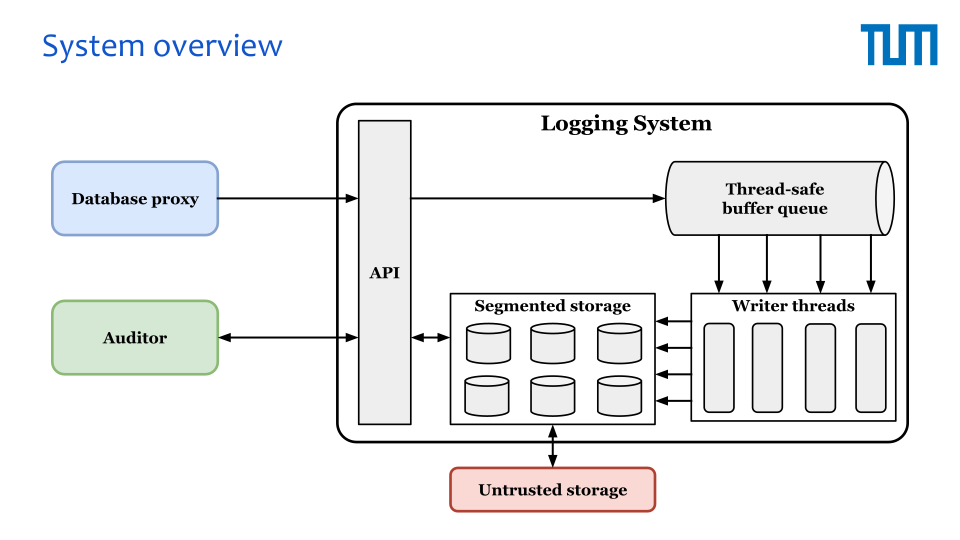
\includegraphics[scale=0.4]{images/systemfigure.png}
    \caption{GDPRlogger system figure}
    \label{fig:systemfigure}
\end{figure}

\section{System Workflow}
The logging process follows a streamlined workflow designed to maximize efficiency and reliability:
\begin{enumerate}
    \item \textbf{Log Entry Creation}: When the GDPRuler engine processes a personal data related operation, it generates a log entry containing relevant metadata such as timestamps, action types, and data locations.
    \item \textbf{Enqueuing}: Log entries are immediately enqueued through the logging API, allowing the calling process to continue without waiting for disk operations.
    \item \textbf{Batch Processing}: Dedicated writer threads continuously monitor the queue, collecting entries into batches for optimized processing.
    \item \textbf{Security Processing}: Batched entries undergo security treatments including compression and encryption, with cryptographic chaining applied to ensure tamper-evidence.
    \item \textbf{Persistent Storage}: Processed batches are written to append-only segment files, with new segments created based on size or time thresholds.
    \item \textbf{Export and Verification}: When required, closed segments can be exported for auditing purposes, with the system performing decryption, decompression, and hash chain verification to ensure data integrity throughout the export process.
\end{enumerate}

\section{System Components}
The logging system consists of four primary components, each serving a specific function.The \textbf{logging API} provides the interface for log entry submission, handling the initial serialization of metadata and ensuring quick response times through asynchronous processing. The \textbf{buffer Queue} acts as the system's central coordination mechanism, implementing a thread-safe, lock-free design to manage the flow of log entries from submission to processing. \textbf{Writer threads} perform the core processing of log entries, managing compression, encryption, and cryptographic chaining while ensuring efficient disk operations through batched writing. The \textbf{segmented storage} manages the physical storage of log data, implementing an append-only design with segment-based organization to facilitate efficient exports and archives while maintaining data integrity.\\

\noindent
Each component is designed to operate independently while maintaining strict coordination through well-defined interfaces. By adhering to these principles and workflows, the logging system achieves the dual goals of high performance and robust GDPR compliance, ensuring that all logged transactions are secure and verifiable.
\input{chapters/04_design}
\input{chapters/05_implementation}
\input{chapters/06_evaluation}
\input{chapters/07_related-work}
\input{chapters/08_summary-conclusion}
\input{chapters/09_future-work}

\appendix{}

\microtypesetup{protrusion=false}

\addchap{Abbreviations}
\begin{acronym}
	\itemsep-.25\baselineskip
	\acro{TUM}[TUM]{Technical University of Munich}
	% TODO: add acronyms
\end{acronym}

\listoffigures{}
\listoftables{}
\microtypesetup{protrusion=true}
\printbibliography{}

\end{document}
